\chapter{LSB Flame Characteristics}
\label{ch:lsb}

Chapter \ref{ch:background} introduced the salient features of the LSB flow field and discussed the mechanisms that enable the LSB to stabilize a flame.
Four flow parameters were introduced that sufficiently describe an operating condition of the LSB---the combustor pressure, \(p\), the preheat temperature, \(T\), the reference velocity, \(U_0\), and the equivalence ratio of the premixed reactants, \(\phi\).
The angle of the swirler vanes, \(\alpha\)---a geometric parameter---was also identified as a variable of interest.
The effect of varying these parameters on the flame characteristics constitutes the subject of this chapter.
The LSB flame was characterized by its location, its shape and its structure.
The first two of these are quantified by the flame standoff distance, \(X_f\), and the flame cone angle, \(\theta_f\) respectively.

In the same chapter, the existing theories explaining LSB operation were outlined.
These theories were developed based on observations of the LSB flame and flow field in experiments conducted at atmospheric pressure, with low velocity, non-preheated reactants.
Restating one objective of this thesis, the goal is to reexamine the validity of these theories at conditions closer to those at which gas turbines operate.

Finally, Chapter \ref{ch:background} examined key parameters that affect each of the flame characteristics, illustrated by the case of varying reference velocity.
The flame location and shape were seen to be controlled by factors affecting the axial velocity profile and the turbulent flame speed.
A Borghi diagram based on turbulence and laminar flame properties was introduced to designate the regime of premixed turbulent combustion that best describes the flame structure.

The following sections examine the results of experimental investigation of the flame characteristics conducted at high preheat and high pressure conditions.

\section{Effect of Reference Velocity}
\label{sec:lsb-effect-of-reference-velocity}


Section \ref{subsubsec:flame-characteristics-standoff} explored how changing the reference velocity is not expected to affect the flame location or the flame shape as the balance between the local reactant velocity and the turbulent flame speed remains unaffected.
This was further borne out by Equation \ref{eqn:chengModel} which outlines a simple model for the turbulent flame speed as a linear function of \(u\) and hence, \(U_0\).
Combined with the self-similar velocity field in the LSB, this predicted that the flame shape and location will be constant over a wide range of operating conditions.
Cheng et al.\cite{2008-cheng-a} reported no significant deviation from this model over the range of conditions at which they tested the LSB design.
It is worth repeating that these experiments were confined to low flow velocities at atmospheric pressure, non-preheated conditions.

In typical gas turbine applications, the reference velocity is not generally variable with engine loading.
Hence, the motivation for studying its effect on the flame characteristics arises from the fact that the reference velocity is a design parameter and its effect on the flame has implications for the design of future LSB-based gas turbine engines.
If the atmospheric pressure model holds at high pressure conditions and the reference velocity has no discernible effect on the flame shape and location, such behavior is desirable from the point of view of a gas turbine designer as it would simplify models for heat transfer and combustor length.

In order to verify the validity of this model at high pressure conditions in the presence of substantial preheat, the LSB was operated at a pressure of 6 atm and the reference velocity was varied from 10 to 40 m/s.
For these tests, the \(S_{37^\circ}\) swirler was used.
In a parallel series of tests, the \(S_{45^\circ}\) swirler was tested at a pressure of 3 atm at reference velocities of 40 and 80 m/s.
The preheat temperature for these tests was about 500 K.
The measured and calculated flow parameters for these conditions are presented in Table \ref{tab:referenceVelocityCases}.
The location of the flame was measured from CH* chemiluminescence images and the results are presented in Figure \ref{fig:referenceVelocityResults}.

\begin{table}
  \caption[Test conditions for Reference Velocity]{Test conditions for Reference Velocity. FIXME}
  \begin{center}
    \begin{tabular}{lcccc}
      Experiment & \(p\) & \(T\) & \(\phi\) & \(U_0\) \tabularnewline
      & atm & K & & m/s \tabularnewline
      \hline\hline
      Chemiluminescence & & & & \tabularnewline
      \hline
      & 6.04 & 525 & 0.57 \(\pm\) 0.02 & 37.3 \tabularnewline
      & 6.03 & 534 & 0.55 \(\pm\) 0.07 & 20.1 \tabularnewline
      & 6.19 & 524 & 0.55 \(\pm\) 0.07 & 18.9 \tabularnewline
      & 6.19 & 493 & 0.51 \(\pm\) 0.16 & 11.7 \tabularnewline
      & & & & \tabularnewline
      & 3.01 & 485 & 0.57 \(\pm\) 0.04 & 36.7 \tabularnewline
      & 3.02 & 523 & 0.57 \(\pm\) 0.02 & 79.5 \tabularnewline
      & & & & \tabularnewline
      CH PLIF & & & & \tabularnewline
      \hline
      & 1.0 & 315 & 0.90 & 21 \tabularnewline
      & 1.0 & 443 & 0.90 & 40 \tabularnewline
      \hline
    \end{tabular}
  \end{center}
  \label{tab:referenceVelocityCases}
\end{table}


\begin{figure}

\begin{subfigure}{\linewidth}
  \centering
  \input{figures/referenceVelocityDistancePlot}
  \caption{Flame standoff distance as a function of the reference velocity}
  \label{fig:referenceVelocityDistance}
\end{subfigure}

\begin{subfigure}{\linewidth}
  \centering
  \input{figures/referenceVelocityAnglePlot}
  \caption{Flame cone angle as a function of the reference velocity}
  \label{fig:referenceVelocityAngle}
\end{subfigure}

\caption[Effect of reference velocity on the flame location and shape]{The plots show the effect of changing the reference velocity on the flame location and flame shape. The \textcolor{blue}{blue} curves are from tests conducted using the \(S_{37^\circ}\) swirler at 6 atm, while the \textcolor{red}{red} curves are from tests using the \(S_{45^\circ}\) swirler at 3 atm.}

\label{fig:referenceVelocityResults}

\end{figure}



There is essentially no systematic variation in the flame standoff distance or the flame angle for the low velocity, \(S_{37^\circ}\) tests.
This is in line with Equation \ref{eqn:flameImmobility}'s prediction and confirms its applicability even at elevated pressure and preheat conditions.

When the \(S_{45^\circ}\) swirler was tested at higher reference velocities, however, the flame location shifted downstream sharply.
This indicates potential limitations to the simple flame stabilization model that may not predict the behavior of the LSB flame at elevated pressures and temperatures, particularly at high reference velocities.

A possible explanation for this observation can be gleaned from considering the effect that increasing the reference velocity has on the turbulent combustion regime in which the LSB combustor operates.
Previous studies have operated the LSB in regimes where Equation \ref{eqn:chengModel} predicts the variation of the turbulent flame speed with \(u\) with reasonably fidelity.
The arguments behind the formulation of Equation \ref{eqn:chengModel} assume that a turbulent flame can be treated as a distorted/wrinkled laminar flame in the presence of large scale, low intensity turbulence.
This assumption is largely true in the wrinkled flame regime and may even be extended apply to a mildly corrugated flame.
However, as we approach large \(\dfrac{ u }{ S_L }\) values and operate in the thin reaction zone---where most gas turbine combustors operate---the flame bears little resemblance to a wrinkled laminar sheet.
Since increasing the reference velocity (and thus \(u\)) traverses the operating point along the vertical axis of the Borghi diagram, it can cause the turbulent combustion regime to change at high values of \(\dfrac{ u }{ S_L }\), resulting in the ``bending effect'' in the \(\dfrac{ S_T }{ S_L }\) vs \(\dfrac{ u }{ S_L }\) diagram.\cite{1996-kobayashi,2006-law}

One way to ascertain the regimes in which the LSB is operated is to image the flame sheet and observe the flame structure.
To that end, the LSB (Configuration B) was tested at atmospheric pressure with preheat temperatures ranging from 300 to 440 K.
Two of these conditions are at temperatures relevant to this discussion and their operating parameters are presented in Table \ref{tab:referenceVelocityCases}.
In order to prevent flame blow off, the equivalence ratio had to be increased to 0.9.
The resulting flame illuminated by an 80 mm tall, 250 \(\mu\)m thick laser sheet from the alexandrite laser and imaged using the PI-MAX 512\(\times\)512 intensified camera equipped with a 50 mm, f/1.4 lens.
The camera was gated to 300 ns centered on the 70 ns laser pulse.
The laser was operated at 10 Hz and the pulse energy was measured to be about 14 mJ for the low velocity case and about 17 mJ for the high velocity case.
A sample frame from each dataset is shown in Figure \ref{fig:referenceVelocityPLIFResults}. 

\begin{figure}

\centering

\hfill
\begin{subfigure}{0.45\linewidth}
  \centering
  \input{figures/referenceVelocityLowVelPLIFImage}
  \caption{\(U_0\) = 21 m/s}
  \label{fig:referenceVelocityLowVelPLIFImage}
\end{subfigure}
\hfill
\begin{subfigure}{0.45\linewidth}
  \centering
  \input{figures/referenceVelocityHighVelPLIFImage}
  \caption{\(U_0\) = 40 m/s}
  \label{fig:referenceVelocityHighVelPLIFImage}
\end{subfigure}
\hfill

\hfill
\begin{subfigure}{0.45\linewidth}
  \centering
  \input{figures/referenceVelocityLowVelPLIFEdge}
  \caption{Intensity edges}
  \label{fig:referenceVelocityLowVelPLIFEdge}
\end{subfigure}
\hfill
\begin{subfigure}{0.45\linewidth}
  \centering
  \input{figures/referenceVelocityHighVelPLIFEdge}
  \caption{Intensity edges}
  \label{fig:referenceVelocityHighVelPLIFEdge}
\end{subfigure}
\hfill

\hfill
\begin{subfigure}{0.45\linewidth}
  \centering
  \input{figures/referenceVelocityLowVelPLIFHistogram}
  \caption{\(\mu\) = 364; \(\sigma\) = 167}
  \label{fig:referenceVelocityLowVelPLIFHistogram}
\end{subfigure}
\hfill
\begin{subfigure}{0.45\linewidth}
  \centering
  \input{figures/referenceVelocityHighVelPLIFHistogram}
  \caption{\(\mu\) = 463; \(\sigma\) = 187}
  \label{fig:referenceVelocityHighVelPLIFHistogram}
\end{subfigure}
\hfill

\caption[Effect of reference velocity on the flame structure]{The sequence of images on the left and the right pertain to the low and high velocity cases respectively. Each instantaneous frame of PLIF data is processed to detect edges and the statistics of the edge pixels from 300 such frames in the central quarter of the image are plotted as a histogram.}

\label{fig:referenceVelocityPLIFResults}

\end{figure}



Both the low and high velocity cases show an essentially unbroken flame sheet that is characterized by wrinkles.
This is consistent with the operating regime being in the wrinkled laminar flame region of the Borghi diagram.
The level of wrinkling in the flame sheet is representative of the increase in the flame area and hence the turbulent flame speed.
This can be quantified by detecting the edges of intensity in these images and measuring the integrated length along the edges.
A simple implementation of this can be done by counting the number of pixels along the intensity edges.
The edge detection algorithm detects two sharp intensity gradients along the flame sheet---one on the reactants side and one on the product side.
Consequently, the flame sheet get doubly counted but this does not affect the statistics as twice the number of edge pixels are counted from all the frames.

The flame sheet also exhibits up-down movement from frame to frame, in addition to wrinkling.
If the statistics are gathered over the entire frame, the up-down motion pollutes the data and the statistics can no longer be attributed to the wrinkling of the flame sheet alone.
To overcome this, edge pixels are counted only over a quarter of the image width, centered on the average flame axis.
The detected edges and histograms of the edge pixels are also presented in Figure \ref{fig:referenceVelocityPLIFResults}.

Figure \ref{fig:velocityFrameSequence} shows three consecutive frames each from the low velocity, low preheat case and the high velocity, high preheat case.
The level of wrinkling is predictably higher for the high velocity, high preheat case.
The instances of disjoint packets of flame are also higher for this case.
This can also be seen in the histogram in Figure \ref{fig:referenceVelocityPLIFResults} where the average number of detected edges in the region of interest is higher for the high velocity case.
The higher instances of finding disjoint packets of flame in high velocity, high preheat case, in particular indicates that the operating point is approaching the boundary between the laminar wrinkled flame regime and the corrugated flame regime.

\begin{figure}

\centering

\hfill
\begin{subfigure}{0.45\linewidth}
  \input{figures/lvframe0}
  \caption{Frame \#0}
  \label{fig:lvframe0}
\end{subfigure}
\hfill
\begin{subfigure}{0.45\linewidth}
  \input{figures/hvframe0}
  \caption{Frame \#0}
  \label{fig:hvframe0}
\end{subfigure}
\hfill

\hfill
\begin{subfigure}{0.45\linewidth}
  \input{figures/lvframe1}
  \caption{Frame \#1}
  \label{fig:lvframe1}
\end{subfigure}
\hfill
\begin{subfigure}{0.45\linewidth}
  \input{figures/hvframe1}
  \caption{Frame \#1}
  \label{fig:hvframe1}
\end{subfigure}
\hfill

\hfill
\begin{subfigure}{0.45\linewidth}
  \input{figures/lvframe2}
  \caption{Frame \#2}
  \label{fig:lvframe2}
\end{subfigure}
\hfill
\begin{subfigure}{0.45\linewidth}
  \input{figures/hvframe2}
  \caption{Frame \#2}
  \label{fig:hvframe2}
\end{subfigure}
\hfill

\caption[Effect of reference velocity on the flame structure - II]{The sequence of instantaneous images on the left are taken at 21 m/s at 315 K. The images on the right are acquired at 40 m/s with a preheat of 443 K. The flame sheet on the right is noticeably more wrinkled.}

\label{fig:velocityFrameSequence}

\end{figure}



While the two tested LSB configurations A and B are somewhat different geometries, the mechanisms affecting the flame structure at the stabilization point are very similar.
Further, the size of the largest eddies in the flow---the integral length scale---should be dominated by the geometry of the swirler which is very similar for both configurations.
As a result, we may even place the operating conditions on the same Borghi diagram and apply what we learnt from the CH PLIF imaging tests to the chemiluminescence cases.
In spite of the leaner equivalence ratio, the effect of the elevated combustor pressure is expected to diminish both the flame speed, \(S_L\), and the flame thickness, \(\delta_f\), placing the operating regime higher (and to the right) on the Borghi diagram.
At a sufficiently large reference velocity, the operating point can transition from the corrugated flame regime into the broken flamelets regime.
Such a transition would not have been possible for a similar increase in reference velocity at atmospheric pressure conditions as the corresponding \(\dfrac{ u }{ S_L }\) values would have been too low.
Transitioning into the broken flamelets regime would cause \(S_T\) to increase at a reduced rate with \(u\) and \(U_0\), resulting in the observed downstream shift of the high pressure LSB flame at high reference velocities.

\section{Effect of Preheat Temperature}
\label{sec:lsb-effect-of-preheat-temperature}

In order to explore the effect of increasing the preheat temperature on the flame location, shape and structure, we begin by mapping the velocity field of the combustor using Laser Doppler Velocimetry (LDV).
The conditions were chosen to study the effect of increasing the preheat temperature on both reacting and non-reacting LSB flow fields.
Further, the study includes both low and high reference velocity cases.
The relevant flow parameters relating to these tests are presented in Table \ref{tab:temperatureCases}.
The test cases are named CN (Cold, Non-reacting), HN (Hot, Non-reacting) and HR (Hot, Reacting) based on their preheat and presence of a flame.
All LDV tests were limited to atmospheric pressure conditions.
Implementing the LDV technique at elevated pressures proved difficult due to beam steering issues, coupled with impractical turn-around times between the successive runs that would be required to obtain sufficient LDV data points for analysis.

\begin{table}
  \caption[Test conditions for studying preheat temperature effects]{The following table lists the conditions at which the LSB flow field was mapped using LDV. These experiments were performed on Configuration A.}
  \begin{center}
    \begin{tabular}{lcccc}
      Case & \(T\) & \(\phi\) & \(U_0\) & \(Re\) \tabularnewline
      & K & m/s & & \tabularnewline
      \hline\hline
      & & & & \tabularnewline
      Cold, Non-reacting (CN) & 300 & - & 30 & 72700 \tabularnewline
      Hot, Non-reacting (HN) & 500 & - & 75 & 75200 \tabularnewline
      Hot, Reacting (HR) & 465 & 0.55 & 30 & 39500 \tabularnewline
      \hline
    \end{tabular}
  \end{center}
  \label{tab:temperatureCases}
\end{table}



The normalized centerline mean and rms axial velocity profiles for the three cases are presented in Figure \ref{fig:temperatureLDVResults}.
The abscissa represents the distance from the virtual origin as defined in Section \ref{subsec:lsb-axial-velocity-profile}.

\begin{figure}

\centering

\input{figures/temperatureLDVResultsPlot}

\caption[Effect of preheat temperature on the LSB flow field - I]{The plot shows results from LDV mapping of the flow field in the LSB. Mean axial velocity profiles are shown for \textcolor{blue}{cold}, \textcolor{green}{hot}, and \textcolor{red}{reacting} flow fields. The rms velocities are shown by dashed lines.}

\label{fig:temperatureLDVResults}

\end{figure}



The results show that increasing the preheat temperature causes the normalized velocity slope to increase.
As noted in Chapter \ref{ch:background}, Cheng et al.\cite{2008-cheng-a} reported that this slope is unaffected by the Reynolds number, \(Re\), of the operating condition.
The results in Figure \ref{fig:temperatureLDVResults} however, show that even though the cases CN and HN have similar \(Re\), their mean velocity profiles have very different slopes.
This indicates that the mean axial stretch in the near field of the LSB flow field is a stronger function of the preheat temperature than \(Re\).

\nomenclature{\(Re\)}{Reynolds number}

The preheat temperature impacts the reacting flow field in the LSB in two ways.
First, a higher preheat temperature increases the kinematic viscosity of the flow.
The mechanism that transports the axial momentum in the radial direction and causes the flow to diverge is driven by viscous effects.
Enhanced viscous effects will result in a steeper decrease in the axial velocity.
Simultaneously, this causes an increased production of turbulent kinetic energy.
Second, global reaction rates increase with temperature, causing the laminar flame speed to increase.
The net result of the increased turbulence and laminar flame speed is that the turbulent flame propagates faster.
As a result of the steeper velocity decay and the increased turbulent flame speed, the flame will be expected to stabilize closer to the inlet of the LSB.

Even assuming that \(S_T\) is constant, these results suggest that at higher preheat temperatures, the flame would stabilize closer to the dump plane because of the faster reactant velocity decay.
In fact, the faster velocity decay produces a higher \(u\) and would increase \(S_T\), further causing the flame standoff location to shift upstream.
This affects the stability of the flame in two ways.
First, the flame is closer to the inlet, resulting in more effective heat transfer from the flame zone into the reactants.
Second, the steeper profiles of \(U\) and \(S_T\) limit any movement of the flame in response to perturbations in the local flow field.
These two characteristics of the preheated flame lead to an intuitive result---the LSB flame behaves more stably at high preheat conditions.

Next, we consider how the flame cone angle is affected by increasing the preheat temperature of the incoming reactants.
None of the data sets cover two otherwise identical operating conditions, but at different preheat temperatures.
As a result, the effect must be postulated using data showing the combined effect of increasing reference velocity and preheat temperature.
Figure \ref{fig:temperatureLDVTransverse} shows the profiles of mean axial velocity measured 15 mm downstream of the inlet using LDv.
These measurements are taken from two orthogonal traverses across the flow field and show the profiles for the CN and HN cases.
The results show that the peak mean axial velocity across the shear layer remains the same regardless of velocity or temperature.
However, the thickness of the shear layer has increased.

\begin{figure}

\centering

\input{figures/temperatureLDVTransversePlot}

\caption[Effect of preheat temperature on the LSB flow field - II]{The plot shows LDV data from two orthogonal traverses (along \(Y\) and \(Z\) axes) performed across the LSB combustor. Mean axial velocity is presented for cold and hot cases (both non-reacting) to highlight the effect of preheat on the mean axial velocity profile through the shear layer. The traverses are performed 15 mm downstream of the inlet and use the \(S_{45^\circ}\) swirler in Configuration A.}

\label{fig:temperatureLDVTransverse}

\end{figure}



The angle of the flame cone is decided by the ratio of the mean velocity in the shear layer and the local turbulent speed of the flame.
We can use this relation and explore the propagation of a change in the parameters as follows.

\begin{align}
  U \sin \theta_f &= S_T \nonumber \\
  \therefore \frac{ \delta \sin \theta_f }{ \sin \theta_f } &= \frac{ \delta S_T }{ S_T } - \frac{ \delta U }{ U }
\end{align}

This shows the competing effects of the \(S_T\) and \(U\) in the shear layer.
Since our LDV data indicates that the peak mean axial velocity actually decreases slightly, while the turbulent flame speed would continue to increase with preheat temperature.
The net result of increasing the preheat temperature would thus cause the flame angle to increase.

Finally, we return to the Borghi diagram to consider the effect of a higher preheat temperature on the flame structure.
On the Y-axis, the exponential dependence of \(S_L\) on temperature will decrease the ordinate of the operating point, while on the X-axis, a slight decrease in the flame thickness will move the point to the right.
Figure \ref{fig:temperatureBorghiDiagram} illustrates the direction of movement of such an operating point.
The down-and-right movement of the operating point drives the flame regime away from broken flamelets and closer towards wrinkled/laminar flames.

\begin{figure}

\centering

\begin{tikzpicture}

% Axes
\draw [->, thick] ( -1, 0 ) -- ++( 9, 0 );
\draw [->, thick] ( 0, -1 ) -- ++( 0, 7 );

% Regimes
\draw [gray] ( 0, 2 ) -- ++( 2, -2 );
\draw [gray] ( 1, 1 ) -- ++( 6, 0 );
\draw [gray, dashed] ( 1, 1 ) -- ++( 4, 4 );
\draw [gray] ( 1, 1 ) -- ++( 6, 2 );
\draw [gray] ( 0, 2 ) -- ++( 6, 2 );

% Labels
\node at ( 0.5, 0.5 ) {\textcolor{gray}{I}};
\node at ( 4.5, 0.5 ) {\textcolor{gray}{II}};
\node at ( 4.5, 1.5 ) {\textcolor{gray}{III}};
\node at ( 3.5, 2.5 ) {\textcolor{gray}{IV}};
\node at ( 1.5, 3.5 ) {\textcolor{gray}{V}};

% Operating points
\draw [fill = red, draw = red] ( 2.5, 1.25 ) circle ( 0.1 );
\draw [->, red] ( 2.5, 1.25 ) -- ++( 0.2, -0.45 );
\draw [red, dashed] ( 2.75, 0.75 ) circle ( 0.1 );

\foreach \x in { 0, ..., 5 }
  \node at ( \x + 1, 0 ) [below] {\textcolor{gray}{\(10^\x\)}};
\foreach \y in { 0, ..., 4 }
  \node at ( 0, \y + 1 ) [left] {\textcolor{gray}{\(10^\y\)}};

\node at ( 3.5, -0.75 ) [below] {\(\dfrac{ L }{ \delta_f }\)};
\node at ( -0.75, 3.5 ) [left] {\(\dfrac{ u }{ S_L }\)};

\node at ( 7, 1 ) [right] {\textcolor{gray}{\(S_L = u\)}};
\node at ( 7, 3 ) [right] {\textcolor{gray}{\(Ka = 1\)}};
\node at ( 6, 4 ) [right] {\textcolor{gray}{\(Ka = 100\)}};
\node at ( 5, 5 ) [above] {\textcolor{gray}{\(Da = 1\)}};

\end{tikzpicture}

\caption[Borghi diagram]{The schematic above is a reproduction of the Borghi diagram from Figure \ref{fig:borghiDiagram}. The response of an operating point to increasing preheat temperature is schematically illustrated. If the initial operating point was in the corrugated flame regime, it would tend towards the laminar flame regime as the flame speed increases and the flame thickness slightly decreases.}

\label{fig:temperatureBorghiDiagram}

\end{figure}



\section{Effect of Swirl}
\label{sec:lsb-effect-of-swirl}

As described in Chapter \ref{ch:background}, the amount of swirl in the LSB flow field is quantified by a swirl number as defined in Equation \ref{eqn:theoreticalSwirlNumber}.
Even though there is no tangential momentum in the core of the LSB flow field where the flame is stabilized, the swirl still exerts influence on the flame characteristics.

The LSB utilizes swirl to enhance the divergence of the flow near the inlet.
Consequently, an increased swirl number results in a sharper deceleration of the reactants and a more upstream stabilization point for the turbulent flame.
This is corroborated by past research\cite{1986-starner,1992-chan} which reporter shorter, wider (higher flame cone angle) flames when the amount of swirl in a combustor was increased.

The results from this investigation are in agreement with this observation.
The higher flame angle and shorter flame standoff may be seen in results like those presented in Figure \ref{fig:referenceVelocityResults} or Figure \ref{fig:pressureResults}, for example.
Operated at identical inlet conditions, the \(S_{45^\circ}\) swirler always stabilizes a flame closer to the inlet and with a larger flame angle compared to the \(S_{37^\circ}\) swirler.

This highlights an interesting trade-off for the designers of LSB-based gas turbine engines.
The \(S_{45^\circ}\) flame is located in a sharply decelerating flow field and as we discussed in Section \ref{sec:lsb-effect-of-preheat-temperature}, this results in a more stable flame, resistant to perturbations in the flow field.
Simultaneously, the presence of the concentrated heat release near the inlet increases the strength of the toroidal recirculation zone present there.
As we shall see in Section \ref{sec:lsb-effect-of-equivalence-ratio}, this recirculation zone can become powerful enough to even cause the flame to attach itself to the lip of the inlet.
Such a strong recirculation zone entrains hot products and retains them longer near the zone of heat release.
This is a recipe for the production of thermal \ce{NO_x}.
While no emission measurements were made as part of this study, it may be reasonably anticipated that the \ce{NO_x} performance of the \(S_{45^\circ}\) swirler will be degraded compared to the \(S_{37^\circ}\) swirler.
The trade-off for gas turbine engine designers is thus between flame stability and emissions performance.

In Configuration A, the theoretical swirl number of the flow field is varied by switching out the swirlers.
The mass flow split of each swirler is estimated from the blockage of the perforated plates covering the central portion of the swirler.
On the other hand, Configuration B not only allows precise knowledge of this mass flow split, but also allows one to vary it in operation.
This offers an alternate way to study the effect of swirl by changing the mass flow split.
Figure \ref{fig:swirlPLIFResults} shows CH PLIF images of the flame sheet for a low and high swirl case.
Also shown are the corresponding histograms measuring the statistics of the edge pixels in the central one-fourth of the flame.
The test conditions for these two cases are presented in Table \ref{tab:swirlCases}.

\begin{figure}

\centering

\hfill
\begin{subfigure}{0.45\linewidth}
  \input{figures/referenceVelocityHighVelPLIFImage}
  \caption{\(S\) = 0.57}
  \label{fig:lowSwirlPLIFImage}
\end{subfigure}
\hfill
\begin{subfigure}{0.45\linewidth}
  \input{figures/highSwirlPLIFImage}
  \caption{\(S\) = 0.62}
  \label{fig:highSwirlPLIFImage}
\end{subfigure}
\hfill

\hfill
\begin{subfigure}{0.45\linewidth}
  \input{figures/referenceVelocityHighVelPLIFHistogram}
  \caption{\(\mu\) = 463; \(\sigma\) = 187}
  \label{fig:lowSwirlPLIFHistogram}
\end{subfigure}
\hfill
\begin{subfigure}{0.45\linewidth}
  \input{figures/highSwirlPLIFHistogram}
  \caption{\(\mu\) = 285; \(\sigma\) = 164}
  \label{fig:highSwirlPLIFHistogram}
\end{subfigure}
\hfill

\caption[Effect of swirl on the flame structure]{The images above show a low and high swirl flame imaged by CH PLIF. These experiments are performed on Configuration B under preheated, atmospheric pressure conditions.}

\label{fig:swirlPLIFResults}

\end{figure}


\begin{table}
  \caption[Test conditions for Swirl]{Test conditions for Swirl. FIXME}
  \begin{center}
    \begin{tabular}{lcccc}
      Case & \(T\) & \(\phi\) & \(U_0\) & \(S\) \tabularnewline
      & K & m/s & & \tabularnewline
      \hline\hline
      Low Swirl & 443 & 0.90 & 40 & 0.57 \tabularnewline
      High Swirl & 434 & 0.91 & 40 & 0.62 \tabularnewline
      \hline
    \end{tabular}
  \end{center}
  \label{tab:swirlCases}
\end{table}



These results show that the flame position is strongly affected by changing the swirl number in this manner.
The reduced flow of reactants through the central portion, coupled with the enhanced divergence induced by the increased swirl flow causes the flame to shift much further upstream.
The reduction in the local reactant velocity also decreases the local turbulence level and accounts for a less convoluted flame sheet.

To conclude, the characteristics of the \emph{Low}-Swirl Burner and its flame are the product of its \emph{low} swirl numbers.
Changing the amount of swirl tends to decrease the flame standoff distance and widen the flame cone angle.
In the limit, when the core flow velocity is too low, the flame can flash back through the swirler.

\section{Effect of Equivalence Ratio}
\label{sec:lsb-effect-of-equivalence-ratio}

The LSB is primarily intended for fuel-lean operation in order to utilize its low \ce{NO_x} emission performance.
As a result, most of the high pressure testing was done as close as possible to a target \(\phi\) of 0.56.
Limited testing was carried out at 12 atm for two off-target conditions: a slightly richer (\(\phi \approx 0.58\)) and a slightly leaner (\(\phi \approx 0.53\)) mixture, in order to explore the sensitivity of the LSB flame to limited changes in equivalence ratio.
The \(S_{45^\circ}\) swirler was used for these tests.
The conditions are presented in Table \ref{tab:equivalenceRatioCases}, while the corresponding averaged and Abel-deconvoluted flame images are presented in Figure \ref{fig:equivalenceRatioResults}.

\begin{table}
  \caption[Test conditions for Equivalence Ratio]{Test conditions for Reference Velocity. FIXME}
  \begin{center}
    \begin{tabular}{lcccc}
      Experiment & \(p\) & \(T\) & \(\phi\) & \(U_0\) \tabularnewline
      & atm & K & & m/s \tabularnewline
      \hline\hline
      & & & & \tabularnewline
      Chemiluminescence & & & & \tabularnewline
      \hline
      & 12.4 & 570 & 0.53 \(\pm\) 0.01 & 39.42 \tabularnewline
      & 12.6 & 583 & 0.58 \(\pm\) 0.01 & 39.42 \tabularnewline
      & & & & \tabularnewline
      CH PLIF & & & & \tabularnewline
      \hline
      & 1.0 & 443 & 0.90 & 40 \tabularnewline
      & 1.0 & 438 & 1.05 & 40 \tabularnewline
      \hline
    \end{tabular}
  \end{center}
  \label{tab:equivalenceRatioCases}
\end{table}


\begin{figure}

\centering

\hfill
\begin{subfigure}{0.45\linewidth}
  \input{figures/leanFlameAverageImage}
  \caption{\(\phi\) = 0.53}
  \label{fig:leanFlameAverageImage}
\end{subfigure}
\hfill
\begin{subfigure}{0.45\linewidth}
  \input{figures/richFlameAverageImage}
  \caption{\(\phi\) = 0.58}
  \label{fig:richFlameAverageImage}
\end{subfigure}
\hfill

\hfill
\begin{subfigure}{0.45\linewidth}
  \input{figures/leanFlameAbelImage}
  \caption{Abel-deconvoluted image}
  \label{fig:leanFlameAbelImage}
\end{subfigure}
\hfill
\begin{subfigure}{0.45\linewidth}
  \input{figures/richFlameAbelImage}
  \caption{Abel-deconvoluted image}
  \label{fig:richFlameAbelImage}
\end{subfigure}
\hfill

\caption[Effect of equivalence ratio on the flame shape - I]{Figures \ref{fig:leanFlameAverageImage}--\ref{fig:richFlameAverageImage} show mean CH* chemiluminescence images of the LSB flame taken at high pressure for two equivalence ratios. Figures \ref{fig:leanFlameAbelImage}--\ref{fig:richFlameAbelImage} show the Abel-deconvolution of the average image highlighting the flame brush. The centerline of the combustor is along the lower edge of the Abel half-images.}

\label{fig:equivalenceRatioResults}

\end{figure}



Two characteristics of the flame are immediately obvious from these images.
First, the zone of heat release, marked by the region from which CH* chemiluminescence is observed, becomes increasingly compact at fuel-rich conditions.
Virtually all other flame images acquired at leaner conditions show a long flame like in Figure \ref{fig:leanFlameAverageImage}, with the heat release distributed over the entire visible area of the combustor.
As discussed in the previous section, a compact heat release zone near the inlet results in strong recirculation features and potentially poor \ce{NO_x} performance, e.g., an even higher \ce{NO_x} increase than would be attributed to just the increase in temperature associated with the higher equivalence ratio.

Second, the flame brush for the richer flame in Figure \ref{fig:richFlameAverageImage} can be observed to wrap around and anchor itself on the dump plane.
This is particularly observable in the Abel-deconvoluted image of the same flame in Figure \ref{fig:richFlameAbelImage}.
The attached region is not as bright as the rest of the flame brush, indicating that the flame may be attaching itself only intermittently.
This intermittent behavior can be confirmed from the instantaneous images where it is visible on some of the acquired images, but not others.
This is seen from the sequence of images shown in Figure \ref{fig:frameSequence}.
This behavior was alluded to in Section \ref{sec:lsb-effect-of-swirl} as being the result of the enhanced toroidal recirculation zone produced by this swirler.
Thus, the intermittent attachment of the flame to the inlet indicates the increased importance of the toroidal recirculation zone in stabilizing the rich flame.

\begin{figure}

\hfill
\begin{subfigure}{0.45\linewidth}
  \centering
  \input{figures/frame90}
  \caption{Frame \#90}
  \label{fig:frame90}
\end{subfigure}
\hfill
\begin{subfigure}{0.45\linewidth}
  \centering
  \input{figures/frame91}
  \caption{Frame \#91}
  \label{fig:frame91}
\end{subfigure}
\hfill

\hfill
\begin{subfigure}{0.45\linewidth}
  \centering
  \input{figures/frame92}
  \caption{Frame \#92}
  \label{fig:frame92}
\end{subfigure}
\hfill
\begin{subfigure}{0.45\linewidth}
  \centering
  \input{figures/frame93}
  \caption{Frame \#93}
  \label{fig:frame93}
\end{subfigure}
\hfill

\hfill
\begin{subfigure}{0.45\linewidth}
  \centering
  \input{figures/frame94}
  \caption{Frame \#94}
  \label{fig:frame94}
\end{subfigure}
\hfill
\begin{subfigure}{0.45\linewidth}
  \centering
  \input{figures/frame95}
  \caption{Frame \#95}
  \label{fig:frame95}
\end{subfigure}
\hfill

\caption[Effect of equivalence ratio on the flame shape - II]{The sequence of frames above is taken from the high equivalence ratio data set and shows the flame intermittently attaching to the lip of the inlet.}

\label{fig:frameSequence}

\end{figure}



It should be noted that the reliance on a toroidal recirculation zone to anchor the flame to the inlet is one of the primary flame stabilization mechanisms used by traditional swirl combustors.
Thus, LSB swirlers with high vane angles tend to behave like traditional swirl combustors at fuel-rich conditions at high pressure.

In order to explore the flame structure of a richer flame, LSB Configuration B was operated at \(\phi\) values of 0.90 and 1.05 and imaged using CH PLIF.
The conditions are listed in Table \ref{tab:equivalenceRatioCases} and the sample instantaneous images from the dataset are presented in Figure \ref{fig:equivalenceRatioPLIFResults}.
The accompanying histograms show statistics of the number of pixels detected on intensity edges.
The average length (or number of edge pixels) of the flame sheet is lower at the higher equivalence ratio.
This implies that the richer flame is less convoluted in the vicinity of the flame stabilization point.

\begin{figure}

\hfill
\begin{subfigure}{0.45\linewidth}
  \centering
  \input{figures/referenceVelocityHighVelPLIFImage}
  \caption{\(\phi\) = 0.90}
  \label{fig:lowEquivalenceRatioPLIFImage}
\end{subfigure}
\hfill
\begin{subfigure}{0.45\linewidth}
  \centering
  \input{figures/highEquivalenceRatioPLIFImage}
  \caption{\(\phi\) = 1.05}
  \label{fig:highEquivalenceRatioPLIFImage}
\end{subfigure}
\hfill

\hfill
\begin{subfigure}{0.45\linewidth}
  \centering
  \input{figures/referenceVelocityHighVelPLIFHistogram}
  \caption{\(\mu\) = 463; \(\sigma\) = 187}
  \label{fig:lowEquivalenceRatioPLIFHistogram}
\end{subfigure}
\hfill
\begin{subfigure}{0.45\linewidth}
  \centering
  \input{figures/highEquivalenceRatioPLIFHistogram}
  \caption{\(\mu\) = 353; \(\sigma\) = 127}
  \label{fig:highEquivalenceRatioPLIFHistogram}
\end{subfigure}
\hfill

\caption[Effect of equivalence ratio on the flame structure]{Instantaneous CH PLIF images of a relatively lean and rich flame at preheated, atmospheric pressure conditions are shown. The histograms show the statistics of the number of detected intensity edges over 300 such frames. These experiments are conducted on Configuration B.}

\label{fig:equivalenceRatioPLIFResults}

\end{figure}



On the Borghi diagram, increasing the equivalence ratio increases the laminar flame speed, and decreases the flame thickness.
Neglecting any associated changes in the velocity field, this causes the operating point to move down and to the right on the diagram, much like in Figure \ref{fig:temperatureBorghiDiagram}.
This change will move the point closer to the wrinkled laminar flame regime, reducing the amount of wrinkling and hence, the length of the flame sheet as demonstrated by the histogram in Figure \ref{fig:equivalenceRatioPLIFResults}

\section{Effect of Combustor Pressure}
\label{sec:lsb-effect-of-combustor-pressure}

In many gas turbine engines, the combustor pressure varies directly with the loading of the engine.
Like the preheat temperature, the combustor pressure affects the LSB flame both through the fluid mechanics of the flow (by decreasing the kinematic viscosity) and the flame's chemical kinetics and scalar diffusion (affecting the laminar flame speed and flame thickness).

There is some confusion over how to study this effect and what to attribute it to.
Pressure effects are often tracked using the Reynolds number.
However, as noted in Section \ref{sec:lsb-effect-of-preheat-temperature}, it might not be the right parameter to use in the near field of the inlet.
According to the turbulent flame speed model from Equation \ref{eqn:chengModel}, at high pressures, the \(S_L\) term is insignificant compared to \(u\) and thus, the turbulent flame speed should see minimal pressure effects.
Indeed, Kobayashi et al.\cite{1998-kobayashi,2002-kobayashi-b} have observed precisely this---the turbulent flame speed appears to be independent of the combustor pressure in their Bunsen burner setup.
While Cheng et al. highlight the diminishing role of \(S_L\), Griebel et al.\cite{2007-griebel} attribute this behavior to the fact that the decrease in laminar flame speed at high pressure is compensated for by the broadening of the turbulence spectrum.
This results in finer turbulent structures in the flow as pressure increases---an observation also made by Kobayashi\cite{1997-kobayashi}---that cause a higher turbulent flame surface area and keep the turbulent flame speed nearly constant.
Griebel et al. further note that theoretically, a slight drop in the turbulent flame speed with pressure may be expected.

In order to resolve the uncertainties regarding how the LSB flame responds to combustor pressure, the flame was imaged over a range of operating conditions from 3 to 12 atm.
For these tests, the reference velocity and the equivalence ratio were held constant.
However, the temperature of the reactants increased somewhat with pressure.
The reason for this was discussed in Chapter \ref{ch:experimental} and is because of the reduced heat losses in the supply lines at the high flow rates required to pressurize the LSB.
The experimental conditions are presented in Table \ref{tab:pressureCases}
The flame location and cone angle inferred from the flame images are presented in Figure \ref{fig:pressureResults}.

\begin{table}
  \caption[Test conditions for studying pressure effects]{The following are the test conditions at which pressure sweeps were performed to study its effects on the flame characteristics. The experiments were conducted on Configuration A and the swirler used for the pressure sweeps is noted.}
  \begin{center}
    \begin{tabular}{lcccc}
      Experiment & \(p\) & \(T\) & \(\phi\) & \(U_0\) \tabularnewline
      & atm & K & & m/s \tabularnewline
      \hline\hline
      & & & & \tabularnewline
      \(S_{37^\circ}\) & & & & \tabularnewline
      \hline
      & 3.06 & 506 & 0.57 \(\pm\) 0.04 & 37.8 \tabularnewline
      & 6.04 & 525 & 0.57 \(\pm\) 0.02 & 37.3 \tabularnewline
      & 9.08 & 544 & 0.56 \(\pm\) 0.02 & 37.2 \tabularnewline
      & 12.1 & 559 & 0.56 \(\pm\) 0.01 & 37.4 \tabularnewline
      & & & & \tabularnewline
      \(S_{45^\circ}\) & & & & \tabularnewline
      \hline
      & 3.01 & 485 & 0.57 \(\pm\) 0.04 & 36.7 \tabularnewline
      & 6.01 & 516 & 0.58 \(\pm\) 0.02 & 38.2 \tabularnewline
      & 9.05 & 553 & 0.58 \(\pm\) 0.01 & 39.2 \tabularnewline
      & 12.0 & 582 & 0.56 \(\pm\) 0.01 & 40.9 \tabularnewline
      \hline
    \end{tabular}
  \end{center}
  \label{tab:pressureCases}
\end{table}


\begin{figure}

\begin{subfigure}{\linewidth}
  \centering
  \input{figures/pressureDistancePlot}
  \caption{Flame standoff distance as a function of the combustor pressure}
  \label{fig:pressureDistance}
\end{subfigure}

\begin{subfigure}{\linewidth}
  \centering
  \input{figures/pressureAnglePlot}
  \caption{Flame cone angle as a function of the combustor pressure}
  \label{fig:pressureAngle}
\end{subfigure}

\caption[Effect of combustor pressure on the flame location and shape]{The plots above show the effect of varying the combustor pressure on the flame location and flame cone angle. The \textcolor{blue}{blue} curves represent data points from the \(S_{37^\circ}\) swirler tests, while the \textcolor{red}{red} curves represent data from the \(S_{45^\circ}\) swirler tests. An uncertainty of \(\pm 1.5\) mm and \(\pm 5^\circ\) are estimated for the standoff distance and flame angle calculations respectively.}

\label{fig:pressureResults}

\end{figure}



At low to moderate pressures, the flame location is nearly invariant for \(S_{37^\circ}\), but moves upstream for the \(S_{45^\circ}\) cases.
This behavior can be explained as follows.
The flame stabilization location for the \(S_{45^\circ}\) swirler is closer to the dump plane compared to the \(S_{37^\circ}\) swirler.
Since the heat transfer back to the reactants is more efficient, the increasing reactant temperature through our test cases dominate pressure effects and moves the \(S_{45^\circ}\) flame upstream.
The \(S_{37^\circ}\) flame is less affected by these processes.

At high pressures, however, both flames are observed to move downstream, despite the increasing preheat temperatures.
The apparent decrease in the turbulent flame speed at these conditions is an unexpected result, and Equation \ref{eqn:chengModel} is insufficient in accounting for this observation.
Figure \ref{fig:pressureResults} also shows that the flame angle for both cases decreases slightly with pressure.
This suggests that the turbulent flame speed was consistently and slowly decreasing with pressure as predicted by Griebel et al.
In light of this, the nearly constant location of the \(S_{37^\circ}\) flame could be attributed to the effects of increasing combustor pressure and preheat temperature nearly canceling each other out at the lower pressures.

This has repercussions for the gas turbine designers as a flame stabilized further away from the inlet is likelier to be blown off due to perturbations.
Increasing the preheat of the reactants could offset this behavior, as can increasing the swirl in the flow field.
In practice, these may be non-trivial to implement in a gas turbine engine.
Adding hydrogen to the reactants may be a simpler way to stabilize the high pressure flames.

Finally, it is interesting to consider this on a Borghi diagram to deduce any changes in the flame structure that might result from high pressure operation.
Kobayashi et al.\cite{1997-kobayashi} report that the increasing pressure causes a weak drop in \(u\), reaching a minimum around 10 atm.
However, the \(\dfrac{ u }{ S_L }\) factor would be dominated by the precipitous fall in the laminar flame speed, causing it to in fact increase with pressure.
On the X-axis, the integral length scale is very nearly unaffected by the pressure change, but the flame thickness decreases rapidly.
Thus, pressure causes the operating point to move up and to the right on the diagram.
This motion is unlikely to cause the turbulent combustion regime to change.
Unfortunately, due to the absence of spatially-resolved, high pressure flame structure images, it may only be surmised at this stage that the observable effect of increasing the combustor pressure would be limited to an increase in the fine structure of the wrinkles in the flame sheet.

\section{Summary of Results}

The effect of various flow parameters on the LSB flame characteristics have been examined using both CH* chemiluminescence imaging and CH PLIF.
The key results from this investigation are as follows:

\begin{enumerate}
  \item Low to moderate reference velocities do not affect the flame at high pressure.
    High reference velocities cause the flame to shift downstream.
    The flame becomes more wrinkled due to increased turbulence.
  \item Preheating the reactants causes the flame to move upstream, but may also strengthen recirculation zones in the combustor.
    The flame structure is expected to become more wrinkled.
  \item Swirl---controlled either through the vane angle or through the mass flow split---causes the flame to anchor closer to the inlet and have a larger cone angle.
    The decreased flow rate through the core reduces wrinkling in the flame structure.
  \item Richer flames at high pressure and high swirl can change flame shape and behave like attached flames.
    Equivalence ratio also results in strong combustion and a less wrinkled flame.
  \item At high pressures, the LSB flame moves downstream.
    In order to preserve flame stability, this should be countered by increasing the preheat or changing the swirl number, if possible.
\end{enumerate}

